\section{Auswertung}
\label{sec:Auswertung}

\subsection{Rote Spektrallinie}
  Es wurden für verschiedene Spektrallinien die Anodenspannung variiert und der resultierende
  Strom zwischen Anode und Anode gemessen. Folgende Werte wurden ermittelt:
  \begin{table}[H]
    \centering
    \caption{Messwerte der roten Spektrallinie}
    \begin{tabular}{c c}
     \toprule
      U [V]& I[nA]\\
     \midrule
      2    & 0.025  \\
      1.75 & 0.02   \\
      1.5  & 0.018  \\
      1.25 & 0.016  \\
      1    & 0.0143 \\
      0.75 & 0.012  \\
      0.5  & 0.01   \\
      0.25 & 0.0075 \\
      0.02 & 0.002  \\
     -0.2  & 0.001  \\
     -0.4  & 0      \\
     -0.6  & 0      \\
     \bottomrule
    \end{tabular}
  \end{table}
  \begin{table}[H]
    \centering
    \caption{Messwerte der grünen Spektrallinie}
    \begin{tabular}{c c}
     \toprule
      U [V]& I[nA]\\
     \midrule
     2    & 1.4  \\
     1.75 & 1    \\
     1.5  & 0.95 \\
     1.25 & 0.8  \\
     1    & 0.7  \\
     0.75 & 0.6  \\
     0.5  & 0.5  \\
     0.25 & 0.4  \\
     0.02 & 0.3  \\
    -0.2  & 0.2  \\
    -0.4  & 0.09 \\
    -0.6  & 0.01 \\
    -0.8  & 0    \\
     1    & 0    \\
     \bottomrule
    \end{tabular}
  \end{table}  
  \begin{table}[H]
    \centering
    \caption{Messwerte der blauen Spektrallinie}
    \begin{tabular}{c c}
     \toprule
      U [V]& I[nA]\\
      \midrule
      2    & 2.1  \\
      1.75 & 1.75 \\
      1.5  & 1.55 \\
      1.25 & 1.4  \\
      1    & 1.23 \\
      0.75 & 1.1  \\
      0.5  & 0.95 \\
      0.25 & 0.8  \\
      0    & 0.7  \\
     -0.2  & 0.5  \\
     -0.4  & 0.3  \\
     -0.6  & 0.2  \\
     -0.8  & 0.15 \\
     -1    & 0    \\
     \bottomrule
    \end{tabular}
  \end{table} 
  \begin{table}[H]
    \centering
    \caption{Messwerte der gelben Spektrallinie im Bereich von 2 V bis -1 V}
    \begin{tabular}{c c}
     \toprule
      U [V]& I[nA]\\
      \midrule
      2    & 0.6   \\
      1.75 & 0.55  \\
      1.5  & 0.5   \\
      1.25 & 0.45  \\
      1    & 0.4   \\
      0.75 & 0.35  \\
      0.5  & 0.28  \\
      0.25 & 0.22  \\
      0.02 & 0.15  \\
     -0.2  & 0.1   \\
     -0.4  & 0.018 \\
     -0.6  & 0     \\
     -0.8  & 0     \\
     -1    & 0     \\
     \bottomrule
    \end{tabular}
  \end{table} 
  \begin{table}[H]
    \centering
    \caption{Messwerte der gelben Spektrallinie im Bereich von 19 V bis -0.2 V}
    \label{tab:idle}
    \begin{tabular}{c c}
     \toprule
      U [V]& I[nA]\\
      \midrule
       19     & 1.43  \\
       18     & 1.4   \\
       17     & 1.37  \\
       16     & 1.3   \\
       15     & 1.27  \\
       14     & 1.26  \\
       13     & 1.25  \\
       12     & 1.2   \\
       11     & 1.19  \\
       10     & 1.17  \\
        9     & 1.1   \\
        8     & 1.07  \\
        7     & 1     \\
        6     & 0.9   \\
        5     & 0.92  \\
        4     & 0.84  \\
        3.5   & 0.78  \\
        3     & 0.72  \\
        2.5   & 0.63  \\
        2     & 0.45  \\
        1.75  & 0.4   \\
        1.5   & 0.32  \\
        1.25  & 0.25  \\
        1     & 0.2   \\
        0.75  & 0.175 \\
        0.5   & 0.12  \\
        0.25  & 0.05  \\
        0.002 & 0.012 \\
       -0.2   & 0     \\
     \bottomrule
    \end{tabular}
  \end{table} 
  Diese Daten sind in Abbildung %\ref{fig:plot} bis \ref{fig:scheisse} dargestellt.
  Für die linearen Teile der Messwerte wurde mittels Python eine lineare Regression 
  anhand der Funktion $\sqrt{I}=aU+b$ angefertigt.

  \begin{figure}
    \centering
    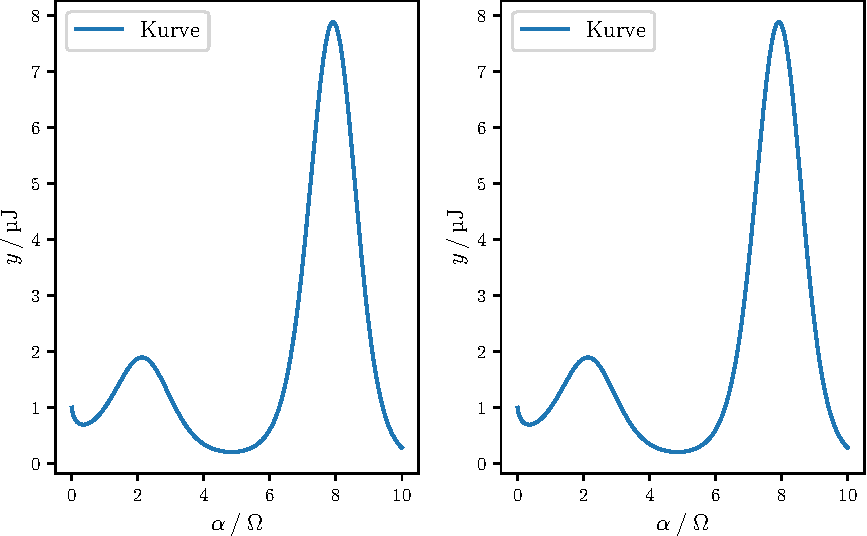
\includegraphics{build/plot.pdf}
    \caption{Messwerte und lineare Regression der roten Spektrallinie}
    \label{fig:plot}
  \end{figure}
  \begin{figure}
    \centering
    \includegraphics{build/fuckyou.pdf}
    \caption{Messwerte und lineare Regression der grünen Spektrallinie}
    \label{fig:fuck}
  \end{figure}
  \begin{figure}
    \centering
    \includegraphics{build/hurensohn.pdf}
    \caption{Messwerte und lineare Regression der blauen Spektrallinie}
    \label{fig:hure}
  \end{figure}
  \begin{figure}
    \centering
    \includegraphics{build/fresse.pdf}
    \caption{Messwerte und lineare Regression der gelben Spektrallinie}
    \label{fig:fresse}
  \end{figure}
  \begin{figure}
    \centering
    \includegraphics{build/verdammtescheiße.pdf}
    \caption{Messwerte und lineare Regression der gelben Spektrallinie}
    \label{fig:scheisse}
  \end{figure}
  
  Die durch die lineare Regression bestimmten Koeffizienten und den Grenzspannungen $U_G$,
  der sich aus den Schnittpunkten mit der Spannungsachse ergibt.
  
  \begin{table}[H]
    \centering
    \caption{Parameter der linearen Regressionen}
    \label{tab:some}
    \begin{tabular}{c c c c}
     \toprule
      $\lambda$ [nm] & a & b & $U_G$ [nV]\\
      \midrule
      614     & 0.106 ± 0.018&0.051 ± 0.005&-0.47867  \\
      577.579 & 0.257 ± 0.015&0.175 ± 0.021&-0.683269 \\
      577.579 & 0.598 ± 0.169&0.395 ± 0.044&-0.660231 \\
      546     & 0.721 ± 0.087&0.561 ± 0.033&-0.77884  \\
      434     & 0.579 ± 0.054&0.817 ± 0.026&-1.41017  \\
     \bottomrule
    \end{tabular}
  \end{table} 
  Durch Umpolen werden die Werte für $U_G$ positiv.
  Aus den erhaltenen Gegenspannungen und Lichtfrequenzen wird erneut eine lineare 
  Regression durchgeführt.
  \begin{figure}
    \centering
    \includegraphics{torte.pdf}
    \caption{}
    \label{fig:torte}
  \end{figure}
  Mit der Ausgleichsgeraden $U_G=a\cdot f +b$ werden die Koeffizienten
  \begin{align*}
    a = (4.46 ± 0.18) \cdot 10^{-15}\\
    b = 1.66 ± 0.1
  \end{align*}
  bestimmt. Die Steigung a entspricht $\dfrac{h}{e}$ und der Achsenabschnitt
  b der Austrittsarbeit in eV. Somit ergibt sich
  \begin{align*}
    h = 4.46 \cdot 10^{-15} eVs\\
    W_A = 1.66 eV.
  \end{align*}
  nachdem die Umrechnung von Nanometern in Metern erfolgt ist.

\subsection{Betrachtung des Photostroms in Abhängigkeit von der Spannung}
  Nun wird bei einer Wellenlänge von $\lambda = 578$ nm der Photostrom bei einer Variation
  der angelegten Brems- bzw. Beschleunigungsspannung von -0.2 V bis 19 V gemessen. Die
  Daten sind in Tabelle \ref{tab:idle} gelistet und in Abbildung \ref{fig:scheiße} dargestellt.
  Es ist ersichtlich, dass es einen Sättigungswert gibt, gegen den die Kurve strebt.
  Dieser kommt durch die konstante Intensität des bestrahlenden Lichtes 
  zustande, da diese proportional zu der Anzahl austretender Elektronen ist.
  Ab einem gewissen Punkt werden nicht mehr Elektronen vom Licht freigesetzt
  als von der Anode angezogen. Der Sättigungswert hängt also nur von der Intensität ab.\\
  Dieser wird asymptotisch angestrebt, da die Elektronen beim Austritt über
  verschiedene kinetische Energien verfügen und daher teilweise die Anode verfehlen,
  weil diese auf einen kleinen Raumbereich beschränkt ist.\\
  Auch bei der Spannung $U_G$ gibt es keinen Knick, sondern eine asymptotische Annäherung.
  Diese exestiert aus dem selben Grund. Auch wenn keine Spannung anliegt, gibt es Elektronen,
  die kinetischische Energie in Richtung der Anode besitzen, sodass trotzdem ein Strom zwischen 
  Kathode und Anode entsteht. \\
  Weiterhin wurde im Bereich der Gegenspannung, also bei $U_G \leq U$ ein entgegengesetzer 
  Stromfluss gemessen. Dieser ist durch die Beschichtung der Kathode zu erklären. Diese
  ist so gewählt, dass diese eine geringe Austrittsarbeit für Elektronen besitzt. Sie 
  verdampft bereits bei geringen Temperaturen, sodass sich ionisierte Atome von der Kathode 
  lösen und aufgrund Ihrer positiven Ladung zur Anode fliegen.\\

%Miks seda ei tööta?